\chapter{Distributed MCTS Algorithms for Cooperating Teams}
\label{chap_dmcts_design}


 The purpose of this chapter is design of distributed coordination algorithms based on
 Monte-Carlo Tree Search. Presented algorithms will work with MCTS tree kept indepentently in
 each cooperative agent. The tree will contain full information about actions done by all
 cooperative agents and also agents from opponent teams. This approach is supposed to be
 appropriate for games with small number of players but with increasing of the number of
 players, the branching factor grows and keeping full MCTS tree turns to be ineffective. The
 tree used in distributed algorithms along with general description of common parts of the
 algorithms are described in Section \ref{sec_dmcts_common}. Before we will propose the
 algorithms description, it is necessary to introduce additional notations for this chapter in
 Section \ref{sec_notations_dmcts} and briefly discuss measures used for comparison of
 distributed algorithms in Section \ref{sec_measures_distributed}. 
 


\section{Useful Notations}
\label{sec_notations_dmcts}

In our algorithms, we will describe, among others, exchange of various parts of the MCTS trees of
the team-mates and it will be useful to give a formal definition of one of them, the so-called
\emph{tree cut}.

\newtheorem*{deftreecut}{Definition}
\begin{deftreecut}[Tree cut]

Let us have a tree $T$ with a set of nodes $N$. \textbf{Tree cut} $C_T$ is a subset of $N$ such that
there is no path between any ascendant $a$ of a node from $C_T$ and any descendant $d$ of a node from
$C_T$ and no node from $C_T$ is an ascendant of any other node from $C_T$. In other words, nodes from a 
tree cut separates a subtree composed of nodes from $C_T$ and
their ascendants from the descendants of nodes from $C_T$. An example of a tree cut is depicted by
Figure \ref{fig_tree_cut_example}.

\begin{figure}
\begin{center}
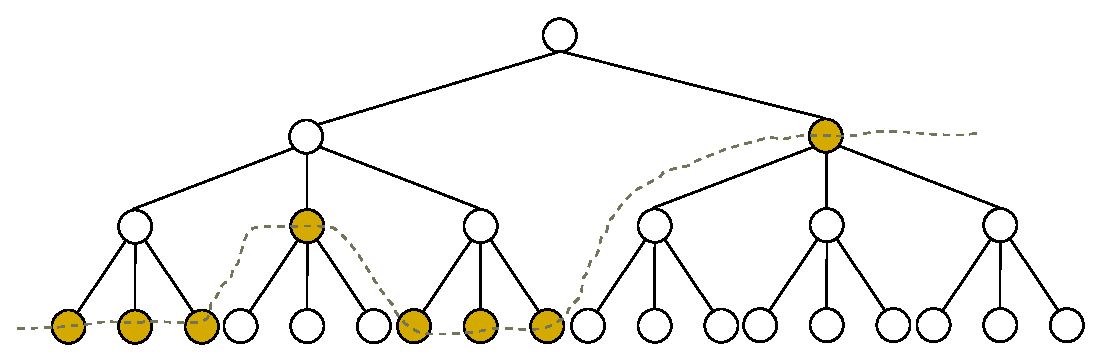
\includegraphics[width=14cm]{img/tree-cut.eps}
\end{center}
\caption{\footnotesize Tree Cut Example.}{\footnotesize Yellow nodes form a tree cut which
separates ascendants and descendants of the nodes of the cut. Each path from root to leaf
contains exactly one node from the cut.}
\label{fig_tree_cut_example}
\end{figure}

\end{deftreecut}





\section{Comparison Measures}
\label{sec_measures_distributed}

Measures suitable for plain Monte-Carlo Tree Search and parallel
Monte-Carlo Tree Search have been already described in Section \ref{sec_measures_parallel}.
We will show that these
measures are also suitable for comparison of distributed MCTS algorithms for games with team
of cooperating agents. In addition, we will compare the amount of communication needed by the
algorithms and the robustness of the algorithms against communication failures. For such
comparisons, we will evaluate strength measures depending on the amount of communication and
its robustness. The amount of communication will be simply the total length of messages
exchanged. Some environments (e.g. radio transmissions or Ethernet over coax) provide the 
possibility of broadcasting messages for the cost of passing single message whereas others 
don't so the cost of broadcasted message equals to the cost of separate messages to all
receivers. We will distinguish between these
environments since some of the algorithms advantage from cheap message broadcasting.

We have described two classes of measures for parallel MCTS, \emph{strength-} and
\emph{simulations-per second-}based measures. Former one works with score obtained at the end
of a game and latter one counts number of MCTS iterations handled per time unit. Details of
these measures are discussed in Section \ref{sec_measures_parallel}. Obviously we can use
simulations-per-second measures, distribution is not obstacle, simulations are still performed
and these measures show the computational costs of distribution of computation. Similar is the
case of strength measures where the only difference is that agents decide the actions
independently but from outer point of view the joint action is the same as if plain or parallel
MCTS calculate action. Strength measures say how strong is team guided by an algorithm.



\section{Proposed Algorithms}

In the following subsections, proposed distributed MCTS algorithms for games with team of cooperative agents
are described together with discussion on their general properties. Since we design algorithms
for distributed MCTS-planning, the algorithms drive particular agents and so all algorithms
have the work \emph{agents} in their name.

\subsection{Backbone of the Distributed Algorithms}
\label{sec_dmcts_common}

\begin{algorithm}
\DontPrintSemicolon
\caption{$DistributedMCTSLoop(tree)$\label{alg_dmcts_common}}
\tcc{general distributed MCTS loop}
\KwData{$tree$\ldots MCTS tree}
\KwResult{$tree$ is enlarged by newly expanded nodes and results of playouts performed are
added. Additional actions are performed during message receiving.
Node representing the best evaluated position reachable by one action is returned}
$i \leftarrow 1$\;
\While(\tcp*[h]{Main MCTS loop}){$EnoughTime()$}{
    \If{$i = 0$}{
        $ReceiveMessages()$\;
    }
    $node \leftarrow Select(tree)$ \tcp*[h]{Phase 1: Selection}\;
    $node \leftarrow Expand(node)$ \tcp*[h]{Phase 2: Expansion}\;
    $rewards[\,] \leftarrow Playouts(node)$ \tcp*[h]{Phase 3: Simulation}\;
    $Backpropagate(tree,node,rewards[\,])$ \tcp*[h]{Ph 4: Backpropagation}\;
    \If{$i = 0$}{
        $SendMessages()$\;
    }
    $i \leftarrow (i + 1)\;\mathrm{mod}\;N_{it}$\;
}
\Return{$\argmax\limits_{n \in Children(root)}c_n$} \tcp*[h]{Return most visited child}\;
\end{algorithm}

MCTS-based agents will iteratively build MCTS tree exactly as plain MCTS algorithm does. In
addition, before certain set of MCTS iterations, the agent receives messages from its team-mates
and performs appropriate actions. Similarly after the set of MCTS iterations, the agent
broadcasts messages to the team-mates. The communicaton between agents is the point differencing
particular distributed algorithms. Algorithms can also differ in other details such as random
seed intialization. Following subsections describe particular distributed algorithms.


\subsection{Independent Agents}

We will first describe the algorithm which is supposed to be the weakest one since no
communication between agents is performed. It serves as lower bound on performance of the
algorithms. The only trick used for the algorithm is setting of the random seed for the
simulation. Because there si no communication between agents, it can easily happen that agents
discovers different local minima. To avoid such a behaviour, the random seed for all agents are
set to same value during agent initialization. And because the agents have equal time to
compute the answer, the size of trees at the end of computation will be similar (this may not
be true for agents with inequal computational strength). If we suppose that all agents
calculate exactly the same number of iterations, time proposed to the agents is $t$ and the 
number of agents is $N$, then the
strength of this algorithm is supposed to be equal to the plain MCTS algorithm with computation
time equal to $t \over N$. This is obvious since the size of the tree of such a plain MCTS
algorithm is equal to trees computed by the independent agents. The only difference is that
independent agents have to calcupate their trees $N$-times since no communication is allowed.

Advantage of the algoritmh is that no communication is needed so it is not affected by
unreliability of the communication network.



\subsection{Joint-Action Exchanging Agents}

Simple way how to synchronize the movement of the agents is exchanging of the messages
containing the information about the actual best joint-action (tuple of actions of all
cooperating agents). The joint-action exchanging agents uses such a synchronization. When it is
a time to decide which action should be played, simple voting is used. Each agent sumarizes
most recent joint-actions received from all team-mates and uses the most frequent one. For
situations when multiple joint-actions with same frequency occurs, ordering on agents is
defined action played by agent higher in the ordering is played. To improve advantages of the
algorithms, different random seeds are used for initialization of the agents and so possibly
different local minima are considered during voting phase.

Such a communication is very low-cost and so does not require wide network channel. Since the
actual best joint-action does not change after very often, we can send the message only when it
is changed to further reduce costs on channel and computations related to networking. For cases
when network is too slow to handle all joint-action messages, all unsent messages (except one
which is being already transmitted) are flushed and the recent one is enqueued.


\subsection{Root Exchanging Agents}
\label{sec_root_exchanging_agents}

Joint-action exchanging agents are voting for the best joint-action but the tree from which the
joint-action is calculated contains only simulations done by the winning agent. Root exchanging
agents increase the strength of chosen action by merging of strengths of all possible 
joint-actions calculated by
all agents and so resulting joint-action is based on results from trees of all team-mates. This
strategy is based on root parallelization algorithm described in Section
\ref{sec_root_parallelization}.

Since the results from trees are merged, we want to build different trees in each action, so 
random seeds
are initialized to different values for each agent. The term "root" in this case means set of
actions $Actions(r)$ playable from the root $r$ of the MCTS tree together with their visit
counts $n_i, i \in Children(r)$. After the root merging, all agents have almost identical
set of joint-action -- visit-count pairs (some differences may occur since not the most recent roots
may be received at time of merging). Joint-action with highest summed visit count is
selected (ordering on joint-actions is used when multiple joint-actions have same visit count).

In case of single-player game, previous description of algorithm works well but there is a little
difficulty when any opponent is considered because set $Children(r)$ may not be a set of actions of
our team. We can simply wait for opponents' turn and exchange our messages during the period
when our team is on turn but this approach has two weaknesses. The first one is that this
perios may be very short what may, along with unreliable networking channel, lead to no
exchanging performed at all. The second weakness is that such a period for message
exchanging may not be present at all in case of turn-based game converted from simultaneous
game if current state was created by splitting simultaneous turn (see Section 
\ref{sec_turn_based_game_conversion}). We resolve this situation by extending definition of the
root for turn-based games with multiple teams. 

For multi-player games, the algorithm will exchange \emph{next-action tree cut} of a player $P$
being on turn. The next-action tree cut is defined as follows:

\newtheorem*{defnextactiontreecut}{Definition}
\begin{defnextactiontreecut}[Next-action tree cut]
Let us have a tree cut $C_1$ composed of nodes in which player $P$ is on turn and which are the first
nodes occuring on the path from tree root to its leaves. For all ascendants $C_1$, any player
different from $P$ is on turn. Then, we will call a set of children of nodes from $C_1$, which
also composes a tree cut, a \textbf{next-action tree cut} for a player $P$.

Algorithm \ref{alg_next_action_tree_cut_construction} describes construction of next-action
tree cut. \todo{Popsat slovně algoritmus}

\end{defnextactiontreecut}

\begin{algorithm}
\DontPrintSemicolon
\caption{$BuildNextActionTreeCut(tree, player)$\label{alg_next_action_tree_cut_construction}}
\tcc{construction of next-action tree cut}
\KwData{$tree$ \ldots MCTS tree \\
$player$ \ldots player constructing }
\KwResult{Algorithm returns the Next-Action Tree Cut of $tree$ for a player $P$}
$C_{curr} \leftarrow \{Root(tree)\}$ \tcp*[h]{cut growing from root}\;
$C_{next\_action} \leftarrow \varnothing$ \tcp*[h]{final next action cut}\;
\While{$C_{curr} \not= \varnothing$}{
    \ForEach{$node \in C_{curr}$}{
        $C_{curr} \leftarrow C_{curr}  \setminus \{node\}$\;
        \eIf{$OnTurn(node)=P$}{
            $C_{next\_action} \leftarrow C_{next\_action} \cup Children(node)$\;
        }{
            $C_{curr} \leftarrow C_{curr} \cup Children(node)$\;
        }
    }
}
\Return{$C_{next\_action}$}
\end{algorithm}

Next-Action Tree Cut is being sent as array containing pairs of visit counts of nodes and
corresponding paths to the nodes represented as list of actions leading to the nodes. For
single-player game case, this approach leads to exchange of set of joint-action -- visit-count
pairs of root's children, how described earlier.

There is another difficulty with exchanging of Next-Action Tree Cut which is that the size of
the cut may grow excessively with growing number of players playing simultaneously so this 
algorithm is not suitable for such games. This fact should be kept in mind
when appropriate algorithm for a particular game is being chosen. When reliable communication
between agents is guaranteed, it is possible to safely exchange the cuts only in turns when the
player is on turn (considering simultaneous nature of the game). In case of unreliable
communication, on the other hand, information contained in cuts from turns when the player is
not on turn can be used with benefit if no communication can be done during the player's turn.


\subsection{Simulation Results Exchanging Agents}

\emph{Simulation Results Exchanging Agents} directly follow the idea of Simulation Results
Passing algorithm described in \ref{sec_simulation_passing}. Since Simulation Results Passing
algorithm is designed for cluster environment, we have to deal with two main differences in
distributed coordination environment which are agents' independent reasoning and limited
and potentially unreliable communication. 

The former difference is simply managed by abandoning
the idea of master thread and letting all agents to play a calculated action. The latter one,
limited communication, is more serious issue. We cannot transmit all simulation calculated is
the channel is too narrow and so we have to choose which of simulation results will be
transmitted. We will prioritize simulation results which are more recent because such results
carry information about the interesting path in the MCTS tree (in comparison with less recent
ones which also carry the interesting path but not so long).

Mechanism of prioritizing of more recent simulation results is realized by message buffer
where, in opposite of common message sending, new messages with simulation results are inserted
at the beginning of the buffer. Once the buffer is full, the least recent messages are thrown
away.


\subsection{Tree-Cut Exchanging Agents}

Root exchanging agents share the information from their MCTS trees by sending messages
containing as little information as possible what spares the capacity of communication
channels but trees contain only calculations done by a particular agent. In opposite,
simulation results exchanging agents share full information about all simulations and so
each particular MCTS tree contains simulations from all agents and if the channel is reliable
and wide enough, it contains full information calculated together by all agents and all
trees are same. This approach, in comparison with root exchanging agents, brings some
advantages and also some disadvantages. 

Main advantage is higher robustness against
communication failures longer than time available for computation of one game step. Since
simulation results are applied into team-mates' trees, they don't vanish after a game step and
not even after several steps. Thanks to UCT mechanism, most of simulations are performed in
subtree which is finally chosen and all these simulations can be used during calculations of
the next action. This is beneficial also if no communication failure occur.

Most serious disadvantage of simulation results passing agents is that it requires wide
communication channel and if it is not available, only a proportional amount of simulations are
exchanged. Second disadvantage is that each received simulation has to be backpropagated
through the tree which requires additional time for computation.

\emph{Tree-cut exchanging agents} algorithm tries to find a compromise between root exchanging 
and simulation results passing. It keeps the advantage of received simulation results stored
directly in MCTS trees but aggregates them adequately to fit the width of the communication
channel. As a side effect of this approach, less calculation with received simulation results
is required.


Root exchanging agents algorithm constructs and sends the next-action tree cut. Similarly the
tree-cut exchanging agents algorithm sends a \emph{visit count tree cut} having following
properties: entire tree cut can be transmitted multiple times during time of one game step and 
visit counts of nodes of the tree cut are similar. Let us denote $C_{cut}$ the number of tree
cuts transmitted per a game step. Then more cuts transmitted per a game step, more
robust our algorithm is and more recent simulations are transmitted - last cut has to be sent
at most $t = {game step length \over C_{cut}}$ seconds before the end of the game step thus 
algorithm regrets transmission of
simulations performed during last $t$ seconds (at least ${ 1 \over C_{cut} }\%$ of simulations
is not transmitted).

Similarly as root exchanging agents, tree-cut exchanging agents send a tree cut once a sending
queue is almost empty (all messages would be sent during next simulation). At that moment, a
tree cut is constructed and pushed at the end of the queue.

We define the visit count tree cut by introducing pseudocode for its construction, Algorithm
\ref{alg_visit_count_tree_cut_construction}. Algorithm starts with a tree cut containing only
the root of the MCTS tree and iteratively selects the node with highest visit count and
replaces the node with its children. The algorithm ends when desired byte size of the tree cut
is reached.

\begin{algorithm}
\DontPrintSemicolon
\caption{$BuildVisitCountTreeCut(tree,byte\_size)$\label{alg_visit_count_tree_cut_construction}}
\tcc{construction of visit count tree cut}
\KwData{$tree\ldots MCTS tree$\\
$byte\_size\ldots desired size of the tree cut in bytes$}
\KwResult{Visit count tree cut of a given tree possible to transmit using less than
$byte\_size$ bytes}
$cut \leftarrow \{Root(tree)\}$ \tcp*[h]{cut growing from root}\;
$curr\_byte\_size \leftarrow ByteSize(Root(tree))$\;
\While{$true$}{
    $most\_visited \leftarrow \argmax_{i \in cut} n_i$\;
    $children \leftarrow Children(most\_visited)$\;
    $curr\_byte\_size \leftarrow curr\_byte\_size + ByteSize(children)$\;
    \If{$curr\_byte\_size>byte\_size$}{
        \textbf{break}\;
    }
    $cut \leftarrow cut \setminus \{most\_visited\} \cup children$\;
}
\Return{$cut$}
\end{algorithm}

Each agent has to keep information about last received tree cut. Once a new tree cut is
received, an algorithm removes previous one from the tree and applies the new one.


\section{Conclusion}
\label{sec_dmcts_comparison}

\todo{Okomentovat scalability trade-off jednotlivých alg.}

In this chapter, we have proposed a total of five synchronization algorithms with various
communication requirements.

\emph{Independent agents} work with no communication at all, being
synchronized only by keeping same random seed for building trees. Such agents cannot exceed
strength speedup value of 1.0 but can be seen as a very simple and unpretentions way of
coordination without sharing of calculated results.

\emph{Joint-Action exchanging agents} are based on very simple idea of coordination based only
on exchanging the best currently calculated action requiring only a little amount of
communication. In addition, the ghosts vote for the action
being played. Thanks to voting mechanism, algorithm, in addition to simple coordination,
chooses between local minima and the best one is chosen. So strength speedup may reach a value
of strength speedup over 1.0 with almost no regret on number of simulations calculated per
second (joint-action exchanging is very trivial operation taking very little time compared to
one simulation).

\emph{Root exchanging agents} is an algorithm strongly inspired by \emph{root parallelization}
of MCTS. Each agent is receiving a list of next joint-actions together visit counts of
corresponding nodes. Just before the end of turn, the visit counts of individual joint actions
are summed (also with agent's visit counts) and the best joint-action is played. This algorithm
is similar to joint-action exchanging agents in the timing of usage of the information.
Joint-action exchanging agetns vote the best action at the end of the turn same as root
exchanging agents does. The difference is in complexity of the information transmitted. 
More complex information transmission requires more communication but the requirements on the
communication channel are still quite low for this algorithm.
Root
exchanging agents are supposed to reach high value of strength speedup since previous
experiments with root parallelization in \cite{Chaslot2008} shows such a results.

First algorithm projecting received messages immediately after their transmission is
\emph{simulation results passing}. The algorithm is exchanging information about each
simulation backpropagating it to all trees. Thanks to it, the trees grow faster and deeper
exploitation can be performed. On the other hand multiple backpropagation of each simulation
brings some regret on the amount of simulations calculated per second. This approach also
requires high amount of communication.

\emph{Tree-cut exchanging agents} is a trial of compromise between previous two algorithm.
Agents are exchanging the results of simulations in aggregated form of \emph{visit count tree
cut}, propagating them to the tree. Aggregation reduces the amount of communication and regret
on simulation calculation in comparison with simulation results exchanging agents. On the other
hand, received simulations are usually backpropagated multiple times so the simulation
calculation regret depends on the parametrization of the algorithm.

In the next chapter, the algorithms are applied to a specific domain of Ms Pac-Man and compared
and evaluated according to the obtained results.
